\documentclass[]{final_report}
\usepackage{graphicx}
\usepackage{hyperref}


%%%%%%%%%%%%%%%%%%%%%%
%%% Input project details
\def\studentname{Colin Smith}
\def\projecttitle{Using RFID to Remember}
\def\supervisorname{Lorcan Coyle}
\def\moderatorname{Your Moderator Name}


\begin{document}

\maketitle
%\tableofcontents\pdfbookmark[0]{Table of Contents}{toc}\newpage

%%%%%%%%%%%%%%%%%%%%%%
%%% Your Abstract here

\begin{abstract}

\textbf{\textsl{RFID has shown to be a useful technology in recent years, especially in areas
such as wearable computing. As this technology becomes more common,
applications are being developed to benefit people in everyday useful ways. This
project proposes to use this technology to aid human memory, and specifically to
help people find lost items. Losing a wallet or a mobile phone is a common
occurrence for most people. Most people could benefit from a system which can
help them locate lost items. Using the system is simple, the project consists of a
bag with a built in RFID system which reads tags on items placed inside it. This
data will be used to help people locate lost items by interacting with a lost and
found application, which is based on human readable cues. For example, �The
user last took their wallet out of their bag at 12:00 along with their car keys�.
The cues are developed based on when items are identified and in what
combinations with other objects. Users could interact with these cues through a
webpage and also receive alerts on potentially lost items. The cues are developed
based on when items are identified and in what combinations with other objects.}}


\end{abstract}
\newpage


%%%%%%%%%%%%%%%%%%%%%%
%%% Acknowledgments

\chapter*{Acknowledgments}

In your Acknowledgments section, give credit to all the people who helped you in your project.

%%%%%%%%%%%%%%%%%%%%%%
%%% Introduction

\chapter{Introduction}

\chapter{\label{chapter2} Background Research}

\section{An Introduction to RFID Technology}

In recent years RFID has become increasingly recognised for its many potential mainstream
applications and uses. There are many types of RFID available each suited to different types
of these in applications. From the highest level RFID can be divided into two classes, active
and passive \cite{intel}. The system I am implementing is based on passive RFID, whereby the RFID
tags do not require their own power source but are instead activated by the reader using
magnetic induction. Active RFID would require each individual tag to have its own built in
power supply which would prove impractical in the context of this project. Using the passive
technique the reader can power the tags and allow them to transmit a signal corresponding to
its unique binary ID \cite{intel}.

\subsection{Chatchayanuson's Kitchen Tracker}

Chatchayanuson et al.'s Kitchen Tracker system system�s goal is to aid everyday tasks,
specifically grocery shopping \cite{ece}. The system consists of stationary RFID readers in a kitchen
and tags placed on key grocery items within it. As items are removed from the kitchen, i.e.,
used or thrown away, the RFID readers are used to identify these items. This data is used to
assist in grocery shopping indicating key items that are needed in the kitchen through realtime
synchronisation with a phone or PDA. These implementations are based on smart home
concepts \cite{ece}. One important point raised by this implementation is that such technologies
should be unobtrusive and blend naturally into our environment.

\subsection {Ubiquitous Memories}

Kawamura et al.�s Ubiquitous Memories is an innovative system designed to augment human
memory through interaction with objects \cite{ubi}. From a hardware perspective the system
consists of a head mounted display over the left eye for displaying video to the user. This eye
piece also incorporates a camera to record user�s activities and experiences. There is an RFID
reader on one wrist to read tagged objects. These are both connected to a remote control for
the system which connects to a hip mounted wearable computer connected to wireless LAN.
The system records the user�s experiences and activities and passes them to a server to be
stored in a video database. Objects related to specific events are RFID tagged. When a tag is
read the system replays a video related to that object, mimicking the behaviour of human
memory. When people touch objects they often recall associated memories \cite{ubi}. Ubiquitous
Memories was tested using memory and recall techniques using different memory aids, one of
which being the Ubiquitous Memories system. This essentially determines the effectiveness
of the system in aiding human memory and also offers insight into alternate ways of
achieving this. This knowledge could be potentially used to refine or augment the system in
the future. Like the kitchen tracker it is important to point out that such a system needs to be
unobtrusive and feel natural in our environment.

\begin{figure}[h]
\centering
\fboxsep 2mm
\framebox{
	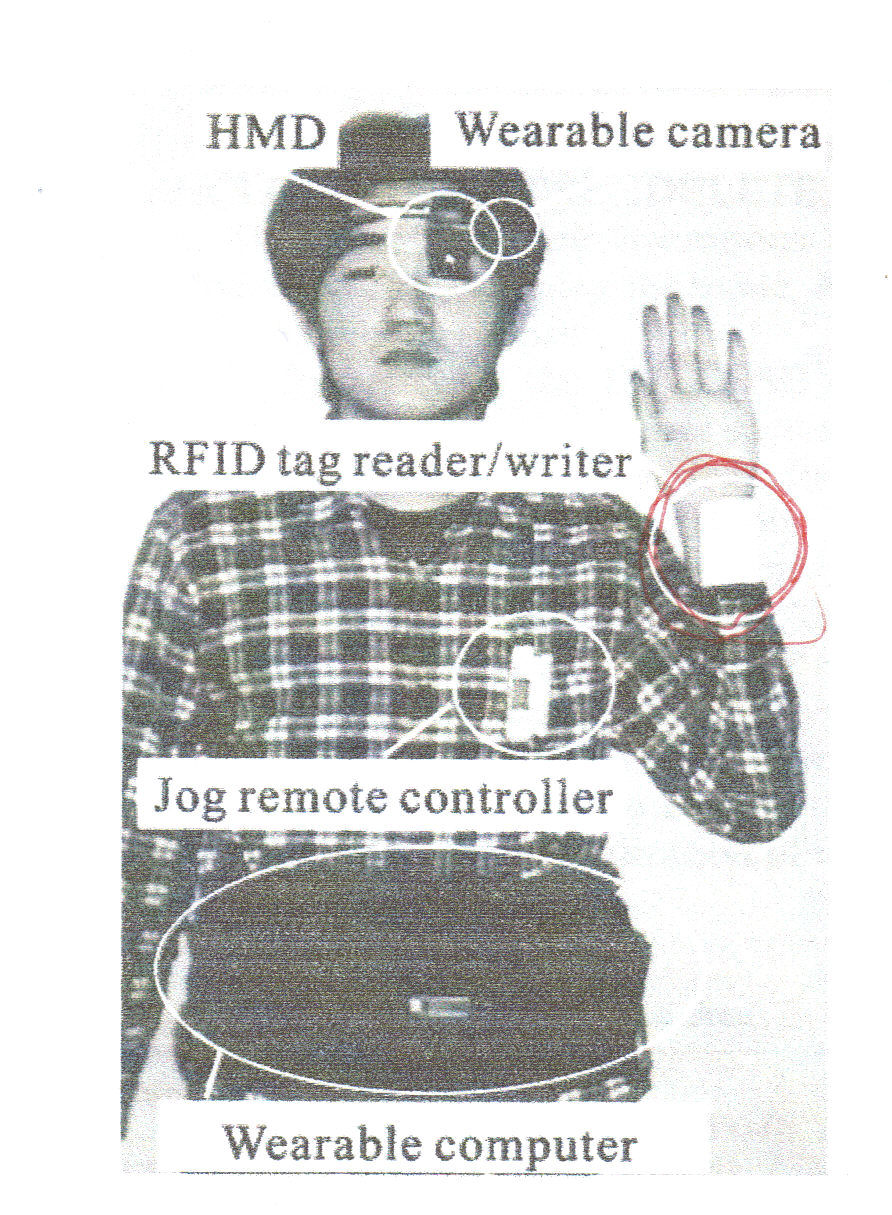
\includegraphics[width=5cm, height=7cm]{borg}
}
\caption{\label{fig:logo} `Ubiquitous Memories` system}

\end{figure} 

\subsection {Schmidt and Gellersen's RFID glove}

Schmidt and Gellersen's RFID glove explores the area of wearable computing where there is
often difficulty in providing computer input if systems carry high cognitive loads or
performance problems in its deployment \cite{schmidt}. Schmidt and Gellersen explore this concept of
human computer interaction using an RFID based system in an attempt to overcome the
inherit shortcomings of wearable computing. The main concept is based on implicit human
computer interaction. Implicit interaction is described as actions which are not primarily
intended to be used as computer input but can still be used as such in some useful way. Their
implementation consists of a glove with an integrated RFID reader. The reader is connected
through a serial connection to a wearable computer. RFID tag IDs are mapped to a specific
URL which increases a counter each time a tag is read. This system is more of a proof of
concept then one with a specific purpose. They conclude that such an implementation
effectively overcomes the traditional problems associated with user input in wearable
computing, and propose that such a system would form a sound base for implementing
practical applications of the technology \cite{schmidt}.

\subsection {Intel Project}

In building useful applications with RFID technology a technique is required in order to allow
the computer to correctly interpret its inputs. How can a task be identified from a set of RFID
readings? In the Intel Seattle iGlove research project the concept of recognising and
interpreting an individual�s activities was explored. Their system prototype was again an
RFID enabled glove with the antenna located in the palm. This is connected to a reader with
radio capabilities for communicating with a computer. The glove components are all housed
in a plastic box on the outer side of the glove, which overall makes the system compact and
unobtrusive. One difficulty their system faced was interpreting `variety�, for example the
same task could be completed in different ways or in a different order of steps. The proposed
solution was to represent tasks in a sequence, or probable sequence, of the objects used,
which resulted in a high level of system accuracy and performance \cite{intel2}.

\begin{figure}[h]
\centering
\fboxsep 1mm
\framebox{
	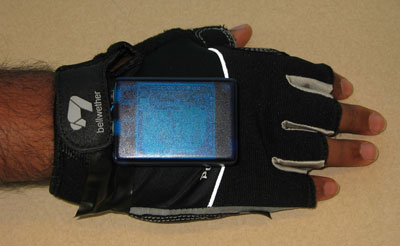
\includegraphics[width=6cm, height=4cm]{iglove} 
	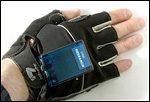
\includegraphics[width=6cm, height=4cm]{iglove2}
}
\caption{\label{fig:logo} Intels `iGlove`}
\end{figure} 

\subsection {Lustig's RFID glove}

Lustig and Coyle developed a similar RFID glove system to the iGlove designed to identify
specific tasks carried out by a user \cite{lustig}. This project is a continuation of this research
attempting to build upon the work already achieved while focusing on a related but slightly
different goal. A glove design was implemented with an RFID reader built into the palm. This
was connected to a Gumstix computer with wireless capabilities. The Gumstix can connect
wirelessly to a server which in turn can update a database of tag reads and pass this
information to a webpage. The system is designed to recognise individual tasks by associating
each one with a number of relevant tags. As my work utilises similar technologies to this
project it will prove useful to take into account the results and findings of their work.

\begin{figure}[h]
\centering
\fboxsep 2mm
\framebox{
	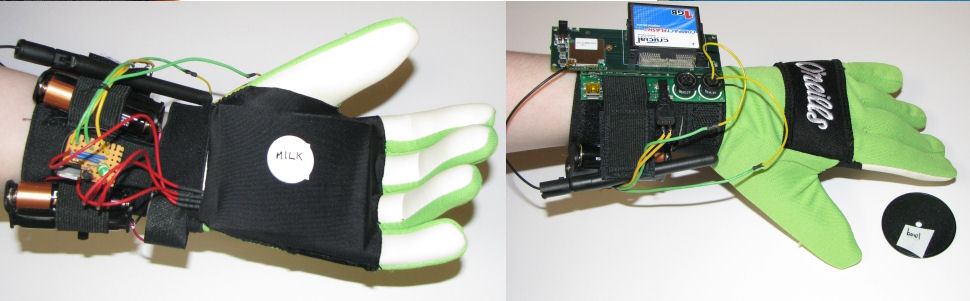
\includegraphics[width=15cm, height=4cm]{lustig}
}
\caption{\label{fig:logo} RFID glove}

\end{figure} 
 
\section{Conclusions}
Much of this previous work in RFID applications offers some guidance for my own work.
One important point raised by many research papers is that such systems need to be
unobtrusive, feel natural to a user, and blend naturally into our environment. Ubiquitous
memories and Chatchayanuson et al.'s kitchen tracker are good examples of this. There are
often many problems in �wearable computing� systems, as discussed by Schmidt and
Gellerson, such as problems with performance. While this is true, it is suggested RFID offers
a sound base for implementing practical applications of these technologies and overcoming
such associated problems \cite{schmidt}. Lustig and Coyle found their RFID system to be very restrictive
\cite{lustig}. This project will explore an alternative form factor in order to overcome these
disadvantages. This project will use the same proven hardware and technologies as Lustig and
Coyle's earlier work, but with a different implementation and application of them.

\chapter{System Implementation}

\section{Hardware Design}

\section{Data Processing}
\newpage

\chapter{System Testing and Evaluation}
\newpage
\chapter{Conclusions and Future Work}
\newpage

%%%% ADD YOUR BIBLIOGRAPHY HERE
\newpage
\begin{thebibliography}{99}
\bibitem{intel}
	  Roy Want,
	  \emph{An Introduction to RFID Technology}.
	  Intel Research, California, 2005.
	  
	\bibitem{intel2}
	  Matthai Philipose, Kenneth P. Fishkin, Mike Perkowitz, Donald J. Patterson, Dieter Fox, Henry Kautz, and Dirk Hahnel,
	  \emph{Inferring Activities from Interactions with Objects}.
	  Intel Research, Seattle, 2004.
	  
	  \bibitem{ece}
	  Suppakrit Chatchayanuson, Charles Christopher Oneyama, Nachiket Shelgikar, Saravana Sivasankaran 
	  \emph{Kitchen Tracker}.
	  Electrical and Computer Engineering, Carnagie Mellon University, 2007.
	  
	  \bibitem{ubi}
	  Tatsuyuki Kawamura, Tomohiro Fukuhara, Hideaki Takeda, Yasuyuki Kono, and Masatsugu Kidode 
	  \emph{Ubiquitous Memories: a memory externalization system using physical objects}.
	  Pers Ubiquit Comput 11: 287-298, 2007
	  
	  \bibitem{smart}
	  Alex S. Taylor, Richard Harper, Laurel Swan, Shahram Izadi, Abigail Sellen, and Mark Perry
	  \emph{Homes that make us Smart}.
	  Springer-Verlag London Limited, 2006
	  
	  \bibitem{cait}
	  Caitlin Lustig, Lorcan Coyle
	  \emph{Reminding Short-Term Memory Sufferers to Complete Routine Tasks}.
	  Technical Report UCD-CSI-2007-10, 2007
	  
	  \bibitem{schmidt}
	  A. Schmidt and C. M. Hans-W. Gellerson
	  \emph{Enabling implicit human computer interaction- a wearable rfid-tag reader}.
	  Proc. 4th Int'l Symp. Wearable Computers (ISWC2000), pp. 193-194
\end{thebibliography}
\label{endpage}



\end{document}

\end{article}
